\documentclass[10pt,a4paper]{book}

\usepackage[utf8]{inputenc}
\usepackage[T1]{fontenc}
\usepackage[french]{babel}
%\renewcommand\sfdefault{phv}
\usepackage[left=2cm, right=2cm, bottom=1.85cm, top=1.5cm]{geometry}
\usepackage[skip=10pt plus1pt, indent=15pt]{parskip}
\usepackage{pgfplots}
\usepackage{fancyhdr}
\usepackage{framed}
\pagestyle{fancy}
\usepackage{hyperref}
\usepackage{multirow}
%\renewcommand{\headrulewidth}{1pt}
%\fancyhead[C]{\textbf{page \thepage}} 
\fancyhead[L]{Cours}
\fancyhead[R]{Terminale STMG}

\renewcommand{\footrulewidth}{1pt}
\fancyfoot[C]{\textbf{page \thepage}} 
\fancyfoot[L]{Lycée Jacques Brel}
\fancyfoot[R]{Année 2022-2023}

%%%%%%%%%%%%%%%%%%%%%%%%%%%%%%%%%%%%%%%%%%%%%%%%%%

%\newcommand{\TDoc}[1]{
%\begin{center}
%{\setlength{\fboxsep}{10pt}  % Ecart texte-boite
%\shadowbox{\textbf{\Large{#1}}}}
%\end{center}
%\vspace{1.5cm}}
    
 \usepackage{fancybox}   %pour l'encadré du titre shadowbox
 \usepackage{stmaryrd}   %pour utiliser correctement les crochets pour les ensembles de définitions
 \usepackage[normalem]{ulem}
 \usepackage{graphicx}
 %\usepackage{wrapfig} %texte coulé autour d'une image
 \usepackage{soul} % souligné
 \usepackage{nonfloat}
 \usepackage[standard]{ntheorem}
 \usepackage{array}
 \usepackage{arydshln}
 \usepackage{graphicx}
%MATHEMATIQUES
\usepackage{amsmath,amsfonts} 
\usepackage{multicol}
\usepackage{tikz}
%%%%% Tableaux de variations
\usepackage{tkz-tab}
%%%%%



\newcommand{\N}{\mathbb{N}}
\newcommand{\Z}{\mathbb{Z}}
\newcommand{\D}{\mathbb{D}}
\newcommand{\Q}{\mathbb{Q}}
\newcommand{\R}{\mathbb{R}}
\newcommand{\Co}{\mathbb{C}}
\newcommand{\K}{\mathbb{K}}
\newcommand{\F}{\mathbb{F}}



%%%%%%%%%%%%%%%%%%%%%%%%%%%%%%%%%%%

\makeatletter
%%%%%%%%%%%%%%%%%%% debut fichier boiboites.sty %%%%%%%%%%%%%%%%%%%%%%
\RequirePackage{xkeyval}
\RequirePackage{tikz}
\usetikzlibrary{intersections}
\usetikzlibrary{positioning}
\usetikzlibrary{3d}
\RequirePackage{amssymb}

\define@key{boxedtheorem}{titlecolor}{\def\titlecolor{#1}}
\define@key{boxedtheorem}{titlebackground}{\def\titlebackground{#1}}
\define@key{boxedtheorem}{background}{\def\background{#1}}
\define@key{boxedtheorem}{titleboxcolor}{\def\titleboxcolor{#1}}
\define@key{boxedtheorem}{boxcolor}{\def\boxcolor{#1}}
\define@key{boxedtheorem}{thcounter}{\def\thcounter{#1}}
\define@key{boxedtheorem}{size}{\def\size{#1}}
\presetkeys{boxedtheorem}{titlecolor = black, titlebackground = white, background = white,%
                         titleboxcolor = black, boxcolor = black, thcounter=, size = .9\textwidth}{}

\newcommand{\couleurs}[1][]{%
    \setkeys{boxedtheorem}{#1}
    \tikzstyle{fancytitle} =[draw=\titleboxcolor, rounded corners, fill=\titlebackground,
                            text= \titlecolor]
    \tikzstyle{mybox} = [draw=\boxcolor, fill=\background, very thick,
                        rectangle, rounded corners, inner sep=10pt, inner ysep=20pt]
}


%Commande generique pour faire un joli encadre
\newsavebox{\boiboite}
\newcommand{\titre}{Titre}
\newenvironment{boite}[2][]%
    {%
    \renewcommand{\titre}{#2}
    \couleurs[#1]
    \begin{lrbox}{\boiboite}%
     \begin{minipage}[!h]{\size}
    }%
    {%
     \end{minipage}
    \end{lrbox}
    \begin{center}
    \begin{tikzpicture}
    \node [mybox] (box){\usebox{\boiboite}};
    \node[fancytitle, right=10pt] at (box.north west) {\titre};
    \end{tikzpicture}
    \end{center}
    }

\newcommand{\newboxedtheorem}[4][]{%
    \couleurs[#1]
    \@ifnotempty{#4}{%
      \@ifundefined{the#4}{\@ifundefined{\thcounter}{\newcounter{#4}}{%
      \newcounter{#4}[\thcounter ] } } { }%
    }
    \newenvironment{#2}[1][]{%
    \@ifnotempty{#4}{\refstepcounter{#4}}
    \begin{boite}[#1]{\textbf{#3\@ifnotempty{#4}{ \csname the#4\endcsname}}\@ifnotempty{##1}{
    (##1)}}
    }%
    {%
    \end{boite}
    }
}

\newcommand{\newboxedtheoreme}[4][]{%
    \couleurs[#1]
    \@ifnotempty{#4}{%
      \@ifundefined{the#4}{\@ifundefined{}{}{%
      } } { }%
    }
    \newenvironment{#2}[1][]{%
    \@ifnotempty{#4}{\refstepcounter{#4}}
    \begin{boite}[#1]{\textbf{#3\@ifnotempty{#4}{ \csname the#4\endcsname}}\@ifnotempty{##1}{
    (##1)}}
    }%
    {%
    \end{boite}
    }
}
%%%%%%%%%%%%%%%%%%%% end fichier boiboites.sty %%%%%%%%%%%%%%%%%%%%%%
\makeatother
\newboxedtheorem{theo}{Théorème}{theorem}
\newboxedtheorem{de}{D\'efinition}{theorem}
\newboxedtheorem{prop}{Propriété}{theorem}
\newboxedtheorem{pro}{Proposition}{theorem}
\newboxedtheorem{ton}{Notation}{theorem}
\newtheorem{exo}{Exercice}
\newboxedtheorem{exe}{Exemple}{theorem}
\newboxedtheorem{cor}{Corolaire}{theorem}
\newboxedtheoreme{conc}{Conclusion}{theorem*}
\newboxedtheoreme{demo}{\textbf{Démonstration guidée}}{theorem}
%%%%%%%%%%%%%%%%%%%%%%%%%%%%%%
%%%%%%%%%%%%%%%%%%%%%%%%%%%%%
\newlength{\longA}
\newlength{\longB}
\newenvironment{BoiteShadow}[3][\linewidth]{%
\addtolength{\longA}{#2}
\addtolength{\longB}{#3}
\begin{Sbox}\begin{minipage}{#1}}%
{\end{minipage}\end{Sbox}%
\setlength{\fboxsep}{\longA}
\setlength{\shadowsize}{\longB}
\shadowbox{\unhbox\@Sbox}\par}
\makeatother
\author{Augustin WENGER}

\title{Cours de Terminale STMG 2 2022-2023}
\date{\today}

%%%% fin du préambule, on passe au contenu : tout le texte entre
%%%% \begin{document} et \end{document} 

\begin{document}
\maketitle
\tableofcontents
\chapter{Suites arithmétiques et géométriques}

\section{Suites : les bases}


\subsection{Vocabulaire}

\begin{de}[Rappel]
    Une \underline{suite numérique} est une liste \textbf{infinie} et \textbf{numérotée} (c'est à dire classée selon un certain ordre) d'éléments.
 Ces éléments sont appelés les \underline{termes} de la suite.
\end{de}


Notation : Si l'on appelle la suite $u$, on note pour tout entier naturel $n$   $u_n$ le $n$-ième terme de la suite.


\textit{Par exemple, si $u$ est la suite des nombres pairs strictement positifs, le $4$-ième terme de la suite est appelé $u_4$ et vaut $8$. On montre les valeurs des termes de cette suite dans le tableau ci dessous }

{
\centering
    \begin{tabular}{|c|c|c|c|c|c|c|c|c|}
        \hline
         $u_1$ & $u_2$ & $u_3$ & $u_4$ & $u_5$ & \ldots & $u_n$ & \ldots\\
        \hline
         $2$ & $4$ & $6$ & $8$ & $10$ & \ldots & $2n$ & \ldots \\ 
        \hline
    \end{tabular}\par
}

Remarque : Une suite est entièrement définie par l'ensemble de ses termes. Si deux suites ont \textbf{tous} leur termes égaux, elles sont égales.

\subsection{Décrire une suite}

Pour exprimer la formule d'une suite, il faut donner une méthode pour calculer chacun de ses termes. Pour cela, deux manières sont possibles :
    \begin{enumerate}
      \item Méthode du \underline{terme général} : On donne directement la formule pour calculer chaque terme. 

      \item Méthode \underline{récursive} : On initialise la suite en donnant le premier terme de la suite, puis on donne une formule pour calculer chacun des termes qui suit en fonction des nombres qui précèdent.
    \end{enumerate}
    
    On peut par exemple dire de la suite $u$ des entiers pairs décrite ci-dessus:
    
      {
      \centering
      Méthode du terme général : \textit{Le terme général de la suite $u$ (définie plus haut) est $u_n=2n$}
      \par

ou
    
      Méthode récursive : \textit{La suite $u$ est définie par $u_1=1$ et pour $n\geq1$, $u_{n+1}=u_n+1$}\par
      }

\subsection{Sens de variation : Suite croissante ou décroissante}

\begin{de}[Rappel]
Une suite est dite \underline{croissante} si ses termes sont de plus en plus grands, c'est à dire si $u_{n+1}$ est \textbf{toujours} supérieur ou égal à $u_n$ quel que soit le choix de l'entier $n$.

On écrit : pour tout $n \geq 1$, $u_{n+1} \geq u_n$
\end{de}

Remarques :
\begin{itemize}
    \item Si on a l'inégalité stricte : pour tout $n \geq 1$, $u_{n+1} > u_n$, on dit que la suite est \underline{strictement} croissante
    \item Si les termes sont de plus en plus petits, c'est à dire si pour tout $n \geq 1$, $u_{n+1} \leq u_n$  on dit que la suite est décroissante.
    \item Pour vérifier si une fonction est (dé)croissante, on regarde si $u_{n+1}$ est plus grand ou plus petit que $u_n$, par exemple en calculant le signe de $u_{n+1} - u_n$. Si le signe est toujours le même, la suite est croissante (si le signe est toujours positif) ou décroissante (si le signe est toujours négatif).
\end{itemize}


Exemple : La suite des entiers pairs $u_n=2n$ est strictement croissante. En effet, pour tout $n \geq 1$, $u_{n+1} - u_n = 2(n+1) - 2n= 2 (n+1-n) = 2 > 0$. $u_{n+1}$ est donc toujours strictement plus grand que $u_n$, ce qui est la définition de la croissance stricte.



\section{Suites arithmétiques}

Intuitivement, les suites arithmétiques sont les suites où pour passer d'un terme à l'autre, on augmente (ou diminue) toujours de la même quantité.

\newcommand{\insertph}[1]{%
 \tikz[remember picture] \node[inner sep=0pt,minimum height=10pt](#1){};} 
 

{
\centering
    \begin{tabular}{|c|c|c|c|c|c|c|c|c|}
        \hline
         $u_1$ & $u_2$ & $u_3$ & $u_4$ & \ldots & $u_n$ & $u_{n+1}$ & \ldots\\
        \hline
         $2\insertph{n1}$ & $\insertph{n2}4\insertph{n3}$ & $\insertph{n4}6\insertph{n5}$ & $\insertph{n6}8$ &  \ldots &  $u_n$\insertph{n7} & $\insertph{n8}u_{n+1}$  & \ldots \\ 
        \hline
    \end{tabular}\par
}

\tikz[remember picture,overlay]\draw[->,blue] ([yshift=-2mm] n1.south) to  [out=-45,in=-150] node[below]{+2} ([yshift=-2mm] n2.south) ; 
\tikz[remember picture,overlay]\draw[->,blue] ([yshift=-2mm]n3.south) to[out=-45,in=-150] node[below]{+2}  ([yshift=-2mm]n4.south); 
\tikz[remember picture,overlay]\draw[->,blue] ([yshift=-2mm]n5.south) to[out=-45,in=-150] node[below]{+2} ([yshift=-2mm]n6.south); 
\tikz[remember picture,overlay]\draw[->,blue] ([yshift=-2mm]n7.south) to[out=-45,in=-150] node[below]{+2} ([yshift=-2mm]n8.south); 


On va voir que cette catégorie de suites a deux caractéristiques importantes :
\begin{itemize}
    \item Elles se retrouvent souvent dans les problèmes concrets :
    \begin{itemize}
        \item On économise de l'argent en plaçant une somme fixe chaque semaine
        \item Un objet s'éloigne d'un autre à une vitesse fixe
    \end{itemize}
    \item On peut facilement obtenir des formules pour calculer un terme donné de la suite, ou même la somme de termes consécutifs de la suite.
\end{itemize}

\subsection{Définition}

\begin{de}
Une \underline{suite arithmétique} est une suite où chaque terme est obtenu en rajoutant le même nombre réel qu'on appelle \underline{raison}) au terme précédent.
Formellement, une suite $u$ est dite géométrique de raison $q$ si pour tout entier $n$ tel que $u_n$ est défini, on a la relation : $u_{n+1} = u_n + r$ 
\end{de}

On déduit de cette définition une première technique pour montrer qu'une suite est arithmétique : On calcule la différence de deux termes consécutifs quelconques : $u_{n+1} - u_n$. Si on trouve quelque chose qui ne dépend \textbf{pas} de $n$, la suite est arithmétique.


\subsection{Propriétés de base}

\begin{prop}

Dans la représentation graphique d'une suite arithmétique, tous les points représentants la suite sont alignés
\end{prop}

\begin{figure}[!h]
  \caption{Exemple : représentation graphique de la suite $u_n=2n$}
    \centering
    \begin{tikzpicture}
      \begin{axis}[ 
        xlabel={n (Numéro du terme)},
        ylabel={$u_n$ (Valeur du terme)},
        xmin=1, xmax=10,
        ymin=0, %ymax=55,
        xtick={1,...,10},
        domain={1:10},
        samples=10
      ]
        \addplot[only marks, mark=x, blue] {2*x}; 
       % \addplot[only marks, red] {21-x}; 
      \end{axis}
    \end{tikzpicture}
\end{figure}

\subsubsection{Calcul du terme général d'une suite arithmétique}

Quand on connaît la raison d'une suite, il suffit de connaître un seul terme et l'on peut calculer tous les termes de la suite :

\begin{prop}

Si on connaît le premier terme $u_1$ d'une suite arithmétique et sa raison $r$, la formule de son terme général est donnée par $u_n=u_1+r(n-1)$.
\end{prop}

Explication : A chaque passage d'un terme à un suivant, on ajoute $r$. Entre $u_1$ et $u_n$, il y a $n-1$ passages. Donc, comme on rajoute $r$ à chaque étape, on obtient un accroissement de $r(n-1)$ au total.

Exemple : $u_1=2$ et $r=2$ (toujours le même exemple). On veut calculer le $5$-ème terme de la suite :

{
\centering
    \begin{tabular}{|c|c|c|c|c|c|}
        \hline
        $u_1$ & $u_2$ & $u_3$ & $u_4$  & $u_5$ & \ldots \\
        \hline
         $2\insertph{n1}$ & $\insertph{n2}4\insertph{n3}$ & $\insertph{n4}6\insertph{n5}$ & $\insertph{n6}8\insertph{n7}$ &  \ $\insertph{n8}10$  & \ldots \\ 
        \hline
    \end{tabular}\par
}

\tikz[remember picture,overlay]\draw[->,blue] ([yshift=-2mm] n1.south) to  [out=-45,in=-150] node[below]{+2} ([yshift=-2mm] n2.south) ; 
\tikz[remember picture,overlay]\draw[->,blue] ([yshift=-2mm]n3.south) to[out=-45,in=-150] node[below]{+2}  ([yshift=-2mm]n4.south); 
\tikz[remember picture,overlay]\draw[->,blue] ([yshift=-2mm]n5.south) to[out=-45,in=-150] node[below]{+2} ([yshift=-2mm]n6.south); 
\tikz[remember picture,overlay]\draw[->,blue] ([yshift=-2mm]n7.south) to[out=-45,in=-150] node[below]{+2} ([yshift=-2mm]n8.south); 
\tikz[remember picture,overlay]\draw[->,red,label = {Lutsa}] ([yshift=-2mm]n1.south) to[out=-100,in=-100] node[below]{$4$ augmentations de $2$ = Augmentation totale de $8$} ([yshift=-2mm]n8.south); 

\vspace{20 mm}

Attention : Si le premier terme n'est pas numéroté $u_1$ mais $u_0$ (ou autre), il faut ajuster le nombre d'étapes pour passer du premier terme à celui qu'on veut calculer.  Par exemple, il y a 5 étapes entre $u_0$ et $u_5$. Plus généralement, entre un terme $u_n$ et un terme $u_N$, avec $n \leq N$ entiers, il y a $N-n$ étapes.

Donc, savoir d'une suite qu'elle est arithmétique \textbf{et} connaître au moins un terme \textbf{et} connaître sa raison suffisent à pouvoir calculer tous les termes de la suite. On dit que ces informations sont \underline{caractéristiques} de la suite (les connaître suffit à connaître la suite dans sa globalité).

C'est même encore plus fort que ça : on peut calculer la raison à partir de la donnée de deux termes de la suite.

\begin{prop}
    Si l'on connaît deux termes distincts $u_n$ et $u_m$ d'une suite arithmétique $u$ (avec $n \neq m$), on peut calculer sa raison $r$ et la formule nous est donnée par : $r = \frac{u_m-u_n}{m-n}$
\end{prop}

Par conséquent, il suffit de connaître 2 informations sur une suite arithmétique pour connaître cette suite :
\begin{itemize}
    \item Sa raison et un terme quelconque
    \item Deux termes quelconques de la suite.
\end{itemize}

\subsubsection{Sens de variation}

Le sens de variation d'une suite arithmétique est intuitivement simple à déterminer : si on augmente entre un terme et le terme suivant (c'est à dire si la raison de la suite est positive), la suite est croissante. Si au contraire on diminue entre un terme et le suivant, la suite est décroissante. Plus précisément :

\begin{prop}
    Si la raison $r$ d'une suite arithmétique est strictement positive, cette suite arithmétique est strictement croissante.
    Si la raison $r$ d'une suite arithmétique est strictement négative, cette suite arithmétique est strictement décroissante.
\end{prop}


On fait le lien avec les fonctions affines : 
\begin{itemize}
    \item Des représentations en points alignés. Mais si on tire un trait ! 
    \item la formule du terme général : $u_n=an+b$ rappelle $f(x)=ax+b$ les fonctions affines ou $y=ax+b$ les équations de droite (non-verticales) du plan
    \item Au même titre que connaître deux points d'une droite permet de caractériser une droite (il existe une et une seule droite passant par deux points), il suffit de connaître deux termes d'une suite pour connaître la suite
    \item La raison, ça fait penser au taux d'accroissement d'une fonction affine (qui est la pente ou le coefficient directeur de la droite), c'est d'ailleurs la même formule, et si l'on connaît sa valeur, il suffit alors d'un terme de la suite (équivalent d'un point d'une droite).
\end{itemize}

\subsection{Moyenne arithmétique}

La moyenne arithmétique de deux nombres réels est ce qu'on appelle couramment la moyenne (mais comme on verra une autre sorte de moyenne, la moyenne géométrique, on précisera désormais de quelle moyenne on parle

\begin{de}
    La \underline{moyenne arithmétique} de deux nombre est la moitié de leur somme, c'est à dire, si l'on note les deux nombres $a$ et $b$, le nombre $\frac{a+b}{2}$
\end{de}

\subsubsection{Lien avec les suites arithmétiques}

On se demande ici si trois nombres $a$,$b$ et $c$ peuvent être trois termes consécutifs d'une suite arithmétique. Pour cela, il faut que l'accroissement entre deux termes soit constant.

{
\centering
    \begin{tabular}{|c|c|c|c|}
        \hline
        $u_1$ & $u_2$ & $u_3$ & \ldots \\
        \hline
         $\hspace{10pt}a\insertph{n1}\hspace{10pt} $ & $\hspace{10pt} \insertph{n2}b\insertph{n3}\hspace{10pt} $ & $\hspace{10pt} \insertph{n4}c \hspace{10pt} $ & \ldots \\ 
        \hline
    \end{tabular}\par
}

\tikz[remember picture,overlay]\draw[->,blue] ([yshift=-2mm] n1.south) to  [out=-45,in=-150] node[below]{$+b-a$} ([yshift=-2mm] n2.south) ; 
\tikz[remember picture,overlay]\draw[->,blue] ([yshift=-2mm]n3.south) to[out=-45,in=-150] node[below]{$+c-b$}  ([yshift=-2mm]n4.south);

Les termes $a$,$b$ et $c$ peuvent être trois termes consécutifs d'une suite arithmétique si et seulement si l'accroissement est constant, c'est à dire si $b-a=c-b$. On peut formuler cela à l'aide de la définition d'une moyenne arithmétique : $b$ doit être "au milieu" de $a$ et de $c$ dans le sens suivant :

\begin{prop}
    Trois nombres $a$,$b$ et $c$ sont trois termes consécutifs (dans cet ordre) d'une suite arithmétique si et seulement si $b$ est la moyenne arithmétique de $a$ et de $c$.
\end{prop}



\subsection{Somme de termes consécutifs d'une suite arithmétique}

En plus de la formule du terme général d'une suite arithmétique, il existe une formule pour calculer la somme des termes consécutifs d'une suite arithmétique :

\begin{prop}
    La somme des termes consécutifs d'une suite arithmétique est égale au nombre de termes dont on fait la somme multipliée par la moyenne arithmétique du premier et du dernier terme.
    Formellement, si $n$ et $p$ sont des entiers avec $n \leq p$, et que $u$ est une suite arithmétique, on a:
    \[  \sum_{i=n}^{p} u_i= u_n + u_{n+1} + \ldots  + u_{p-1} + u_p = \frac{(u_n+u_p)}{2} \times (p-n+1)
    \]
\end{prop}

Explication : N'importe quelle somme de nombres est toujours égale à la moyenne de ses termes multipliée par le nombre de termes (par définition de la moyenne). Or, dans le cas d'une suite arithmétique, les termes augmentent (ou diminuent) toujours de la même quantité, par conséquent si l'on "groupe" les termes en associant le premier au dernier, le deuxième à l'avant-dernier, on obtient toujours la même somme. On peut le voir en utilisant les formules données plus haut si l'on suppose que la raison est $r$:


\begin{tabular}{ccccc}
$u_n + u_p $&$=$ &$  u_n  +  u_n + (p-n) \times r $&$=$ & $ 2u_n + (p-n)r$ \\
$u_{n+1} + u_{p-1} $&$=$&$u_n + r  +  u_n + (p-1-n) \times r $&$=$&$2u_n + (p-n)r$
\end{tabular}

Et ainsi de suite pour tous les termes. On peut donc "retourner" la suite et l'ajouter à elle même, et l'on obtient alors une suite de termes constants, comme l'illustre la figure  \ref{fig:sumarith}

\begin{figure}[htbp]
\centering
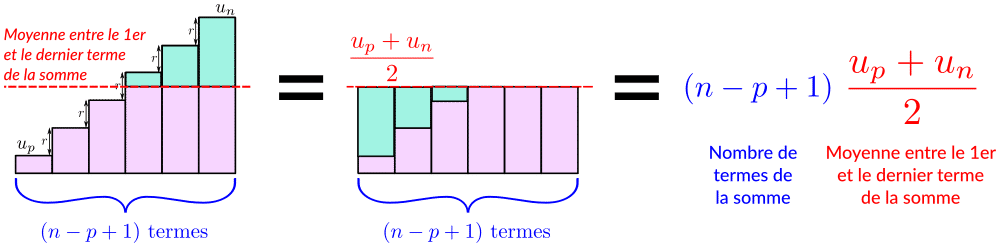
\includegraphics[width=1.0\textwidth]{suites-arithmetiques-somme.png}
\caption{Illustration du principe de la somme de termes d'une suite arithmétique de raison r}
\label{fig:sumarith}
\end{figure}


A retenir :

\begin{itemize}
    \item Mots à savoir définir : suite arithmétique, raison d'une suite arithmétique, moyenne arithmétique
    \item La définition d'une suite arithmétique : permet de vérifier si une suite est arithmétique ou non
    \item La formule du terme général : $u_n = u_1 + (n-1) \times r$
    \item Trouver la raison d'une suite arithmétique à partir de deux termes distincts donnés
    \item Formule de la somme de termes consécutifs d'une suite arithmétique.
\end{itemize}



\section{Suites géométriques}

Pour passer d'un terme au suivant dans une suite géométrique, on ajoutait toujours la même quantité, qui était la raison de la suite. Pour passer d'un terme au terme suivant dans une suite géométrique, on va toujours \textbf{multiplier} par la même quantité : dans l'exemple ci-dessous, on multiplie un terme par 2 pour passer au suivant.


{
\centering
    \begin{tabular}{|c|c|c|c|c|c|c|c|c|}
        \hline
         $u_1$ & $u_2$ & $u_3$ & $u_4$ & \ldots & $u_n$ & $u_{n+1}$ & \ldots\\
        \hline
         $2\insertph{n1}$ & $\insertph{n2}4\insertph{n3}$ & $\insertph{n4}8\insertph{n5}$ & $\insertph{n6}16$ &  \ldots &  $u_n$\insertph{n7} & $\insertph{n8}u_{n+1}$  & \ldots \\ 
        \hline
    \end{tabular}\par
}

\tikz[remember picture,overlay]\draw[->,blue] ([yshift=-2mm] n1.south) to  [out=-45,in=-150] node[below]{$\times 2$} ([yshift=-2mm] n2.south) ; 
\tikz[remember picture,overlay]\draw[->,blue] ([yshift=-2mm]n3.south) to[out=-45,in=-150] node[below]{$\times 2$}  ([yshift=-2mm]n4.south); 
\tikz[remember picture,overlay]\draw[->,blue] ([yshift=-2mm]n5.south) to[out=-45,in=-150] node[below]{$\times 2$} ([yshift=-2mm]n6.south); 
\tikz[remember picture,overlay]\draw[->,blue] ([yshift=-2mm]n7.south) to[out=-45,in=-150] node[below]{$\times 2$} ([yshift=-2mm]n8.south);

On va voir qu'on va pouvoir obtenir comme dans le cas des suites arithmétiques des formules pour calculer le terme général d'une telle suite, son sens de variation, et la somme de termes consécutifs. Certaines formules ressembleront à celles des suites arithmétiques, d'autres moins.

Mais d'abord, petit rappel sur les différentes manières de parler d'une évolution multiplicative.

\subsection{Différentes manière d'exprimer une progression multiplicative}

Il existe plusieurs manières d'exprimer qu'une quantité est multipliée par un certain nombre.

Par exemple, si le prix d'un manteau passe de 100€ à 80€ dans une période de soldes, on peut dire que le prix baisse de 20€ (c'est la vision en \textbf{variation absolue}. On peut dire l'une des  choses suivantes si l'on adopte une vision multiplicative :

\begin{itemize}
    \item Le prix du manteau diminue de 20\%, on dit que $-20\%$ est son \textbf{taux d'évolution}
    \item Le prix du manteau est multiplié par un \textbf{coefficient multiplicateur} de $0{,}8$
\end{itemize}

\begin{de}
    Soit une quantité observée, qui passe d'une valeur initiale VI à une valeur finale VF.
    \begin{itemize}
        \item La \underline{variation absolue} est donnée par $VF - VI$ (vision additive)
        \item Le \underline{taux d'évolution} est donné par $\frac{VF-VI}{VI}$ (On l'exprime souvent en pourcentage)
        \item Le \underline{coefficient multiplicateur} est donné par 
        $\frac{VF}{VI}$. C'est le nombre par lequel on multiplie VI pour obtenir VF.
    \end{itemize}
\end{de}

\begin{prop}
    Pour passer du coefficient multiplicateur au taux d'évolution, on retire $1$ au coefficient multiplicateur. \newline
    Pour passer du taux d'évolution au coefficient multiplicateur, on rajoute $1$ au taux d'évolution.
\end{prop}

\subsubsection{Evolutions successives}

Si deux évolutions successives ont lieu, \textbf{l'évolution totale a pour coefficient multiplicateur le produit des coefficients multiplicateurs.}

Par exemple, une hausse du prix du gaz de 10\% (Coefficient multiplicateur de $1{,}1$) suivie d'une hausse de 50\% ((Coefficient multiplicateur de $1{,}5$) correspond à un coefficient multiplicateur total de $1{,}1 \times 1{,}5 = 1{,}65$ soit une hausse de 65\%


{
\centering
    \begin{tabular}{|c|c|c|c|}
        \hline
        Année& 1 & 2 & 3 \\
        \hline
         Prix du gaz (base 100 en année 1)& $\insertph{n0}100\insertph{n1}$ & $\insertph{n2}110\insertph{n3}$ & $\insertph{n4}165\insertph{n5}$  \\ 
        \hline
    \end{tabular}\par
}

\tikz[remember picture,overlay]\draw[->,blue] ([yshift=-2mm] n1.south) to  [out=-45,in=-150] node[below]{$\times 1{,}1$} ([yshift=-2mm] n2.south) ; 
\tikz[remember picture,overlay]\draw[->,blue] ([yshift=-2mm]n3.south) to[out=-45,in=-150] node[below]{$\times 1{,}5$}  ([yshift=-2mm]n4.south); 
\tikz[remember picture,overlay]\draw[->,red,label = {Lutsa}] ([yshift=-2mm]n0.south) to[out=-100,in=-100] node[below]{$\times 1{,}65$} ([yshift=-2mm]n5.south); 

\vspace{1cm}
En particulier, si le coefficient multiplicateur $q$  est le même sur les $2$ périodes, le coefficient multiplicateur total sera de $q^2$. S'il y a $n$ périodes (avec $n \in \mathbb{N}$), et une multiplication par $q$ à chaque fois, on aura une augmentation totale de $q^n$.

\subsubsection{Evolution réciproque}

Pour calculer l'évolution inverse d'une augmentation en pourcentage, il est pratique de passer par la vision en coefficient multiplicateur. Par exemple, une augmentation de $25\%$ correspond à une multiplication par $1{,}25$. Pour faire l'évolution inverse, on divise par $1{,}25$, car la division par $1{,}25$ est l'opération réciproque d'une multiplication par ce même nombre. Or, une division par $1{,}25$ correspond à une multiplication par $0{,}8$ (car $\frac{1}{1{,}25}=0{,}8$. On repasse alors à la vision en pourcentage : une multiplication par $0{,}80$ correspond à une baisse de $20\%$. $-20\%$ est donc l'évolution réciproque de $+25\%$.



{
\centering
    \begin{tabular}{|c|c|}
        \hline
        $\insertph{n0}100\insertph{n1}$ & $\insertph{n2}110\insertph{n3}$\\ 
        \hline
    \end{tabular}\par
}

\tikz[remember picture,overlay]\draw[->,blue] ([yshift=1mm] n1.north) to  [out=45,in=150] node[above]{\'Evolution de $+25\% = \times 1{,}25$} ([yshift=1mm] n2.north) ; 
\tikz[remember picture,overlay]\draw[<-,red] ([yshift=-2mm] n1.south) to  [out=-45,in=-150] node[below]{$\div 1{,}25 = \times \frac{1}{1{,}25}= \times 0{,}8 =$ \'Evolution de $-20\%$} ([yshift=-2mm] n2.south) ; 

\begin{de}
    L'\underline{évolution réciproque} de l'évolution passant de $VI$ à $VF$ est l'évolution permettant de passer de $VF$ à $VI$. \textbf{L'évolution réciproque possède un coefficient multiplicateur inverse de celle dont elle est la réciproque}
\end{de}

\subsection{Définition d'une suite géométrique}

\begin{de}
Une \underline{suite géométrique} est une suite où chaque terme est obtenu en multipliant par le même nombre réel qu'on appelle \underline{raison}) le terme précédent.
Formellement, une suite $u$ est dite géométrique de raison $q$ si pour tout entier $n$ tel que $u_n$ est défini, on a la relation : $u_{n+1} = u_n \times r$ 
\end{de}

Remarques :
\begin{itemize}
    \item Nous verrons surtout cette année les suites géométriques à terme positifs, qui ont donc une raison positive, c'est à dire $q \in \mathbb{R}^+$
    \item Diviser un nombre par $x$, c'est le multiplier par $\frac{1}{x}$. La définition ci-dessus (qui ne parle que de multiplication) couvre donc tous les cas.
    \item On voit que le mot "raison" n'a pas exactement le même sens que dans le cadre d'une suite arithmétique
\end{itemize}

On déduit de cette définition une première technique pour montrer qu'une suite est géométrique : On calcule le quotient de deux termes consécutifs quelconques : $\frac{u_{n+1}}{u_n}$. Si on trouve quelque chose qui ne dépend \textbf{pas} de $n$, la suite est géométrique.



\subsection{Propriétés de base : Calcul du terme général d'une suite géométrique}

Quand on connaît la raison d'une suite géométrique, il suffit de connaître un seul terme et l'on peut calculer tous les termes de la suite :

\begin{prop}

Si on connaît le premier terme $u_1$ d'une suite géométrique et sa raison $q$, la formule de son terme général est donnée par $u_n=u_1+q^{n-1}$.
\end{prop}
terme
Explication : A chaque passage d'un terme à un suivant, on multiplie par $q$. Entre $u_1$ et $u_n$, il y a $n-1$ passages. Donc, une multiplication totale par $q^{n-1}$.

Exemple : $u_1=2$ et $r=q$ (toujours le même exemple). On veut calculer le $5$-ème terme de la suite :

{
\centering
    \begin{tabular}{|c|c|c|c|c|c|}
        \hline
        $u_1$ & $u_2$ & $u_3$ & $u_4$  & $u_5$ & \ldots \\
        \hline
         $2\insertph{n1}$ & $\insertph{n2}4\insertph{n3}$ & $\insertph{n4}8\insertph{n5}$ & $\insertph{n6}16\insertph{n7}$ &  \ $\insertph{n8}32$  & \ldots \\ 
        \hline
    \end{tabular}\par
}

\tikz[remember picture,overlay]\draw[->,blue] ([yshift=-2mm] n1.south) to  [out=-45,in=-150] node[below]{$\times 2$} ([yshift=-2mm] n2.south) ; 
\tikz[remember picture,overlay]\draw[->,blue] ([yshift=-2mm]n3.south) to[out=-45,in=-150] node[below]{$\times 2$}  ([yshift=-2mm]n4.south); 
\tikz[remember picture,overlay]\draw[->,blue] ([yshift=-2mm]n5.south) to[out=-45,in=-150] node[below]{$\times 2$} ([yshift=-2mm]n6.south); 
\tikz[remember picture,overlay]\draw[->,blue] ([yshift=-2mm]n7.south) to[out=-45,in=-150] node[below]{$\times 2$} ([yshift=-2mm]n8.south); 
\tikz[remember picture,overlay]\draw[->,red,label = {Lutsa}] ([yshift=-2mm]n1.south) to[out=-100,in=-100] node[below]{$4$ multiplications par $2$ = multiplication totale par $2^4 = 16$} ([yshift=-2mm]n8.south); 

\vspace{20 mm}

Attention : Si le premier terme n'est pas numéroté $u_1$ mais $u_0$ (ou autre), il faut ajuster le nombre d'étapes pour passer du premier terme à celui qu'on veut calculer.  Par exemple, il y a 5 étapes entre $u_0$ et $u_5$. Plus généralement, entre un terme $u_n$ et un terme $u_N$, avec $n \leq N$ entiers, il y a $N-n$ étapes.

On a donc la même propriété qu'on avait à la partie précédente : savoir d'une suite qu'elle est géométrique \textbf{et} connaître au moins un terme \textbf{et} connaître sa raison suffisent à pouvoir calculer tous les termes de la suite.

On peut également calculer la raison à partir de deux termes consécutifs de la suite  (on peut à peu près le faire avec deux termes distincts quelconques mais on ne verra pas cette formule ici) :


\begin{prop}
    Si l'on connaît deux termes distincts $u_1$ et $u_2$ d'une suite géométrique $u$, la raison $q$ de cette suite est donnée par $\frac{u_2}{u_1}$
\end{prop}

Comme pour les suites arithmétiques, il suffit donc de connaître deux informations sur une suite géométrique à termes positifs pour connaître toute la suite.

Et c'est la grande utilité de ces deux types de suites : \textbf{Elles permettent d'extrapoler} (prévoir les termes qui suivent) \textbf{ou d'interpoler} (retrouver des termes intermédiaires) \textbf{à partir de deux observations seulement.}

\subsubsection{Sens de variation}

Le sens de variation d'une suite géométrique à termes positifs est là encore plutôt simple à déterminer si l'on connaît les règles de multiplication d'un nombre positif: si on multiplie entre un terme et le terme suivant (c'est à dire si la raison de la suite est plus grande que 1), la suite est croissante. Si au contraire on multiplie par un nombre négatif entre un terme et le suivant, la suite est décroissante. Plus précisément, pour une suite géométrique dont le premier terme $u_1$ est strictement positif :

\begin{prop}
    $q>1$: Si la raison $q$ d'une suite géométrique à termes positifs est strictement plus grande que $1$, cette suite est strictement croissante.
    $0<q<1$ : Si la raison $q$ d'une suite géométrique à termes positifs  est strictement plus petite que $1$ mais plus grande que $0$, cette suite est strictement décroissante.
\end{prop}

Remarques : \begin{itemize}
    \item $q=1$ : Si la raison est \textbf{égale à 1}, la suite est constante.
    \item $q=0$ : Si la raison est \textbf{égale à 0}, tout terme de la suite sera égal à $0$, (sauf son premier terme).
    \item $q<0$ : Si la raison est \textbf{strictement négative}, le sens des termes alternera entre positif et négatif, donc la suite ne sera ni croissante ni décroissante
    \item Si le premier terme d'une suite est négatif au lieu d'être positif, le sens de variation de la suite sera inversé. Par exemple, ne suite géométrique qui commence par $-1$ et a pour raison $2$ deviendra de plus en plus petite, car multiplier un nombre négatif par un nombre plus grand que $1$ le rendra plus petit.
\end{itemize}




\subsection{Moyenne géométrique}

On va voir ici une autre sorte de moyenne de deux nombres : la moyenne géométrique. Le but de la moyenne géométrique est de trouver la formule qui rende juste la phrase suivante :   \textit{Si je multiplie un nombre par a puis par b, cela revient à multiplier par la moyenne géométrique de a et b deux fois.}

Si j'appelle $M$ la moyenne géométrique de deux nombres \textbf{positifs} $a$ et $b$, Je veux que $1 \times a \times b= ab$ soit égal à $1 \times M \times M = M^2$. Cette moyenne doit également être positive.

Or, l'unique valeur positivede $M$ telle que $ab=M^2$ est, par définition de la racine carrée : $M = \sqrt{ab}$

Par exemple,  si $a= 3$ et $b=12$, leur moyenne géométrique est de $\sqrt{3 \times 12} = \sqrt{36} = 6$. 

\begin{de}
    La moyenne géométrique de deux nombres positifs $a$ et $b$ est le nombre $\sqrt{ab}$
\end{de}

On a bien, quel que soit le nombre de départ $x$ : 
\begin{tabular}{ccc}
{
    \begin{tabular}{|c|c|c|}
        \hline
         $x\insertph{n1}$ & $\insertph{n2}ax\insertph{n3}$ & $\insertph{n4}abx$\\ 
        \hline
    \end{tabular}\par
} &et &{\begin{tabular}{|c|c|c|}
        \hline
         $x\insertph{n5}$ & $\insertph{n6}\sqrt{ab}x\insertph{n7}$ & $\insertph{n8}abx$\\ 
        \hline
    \end{tabular}\par
}
\end{tabular}
\tikz[remember picture,overlay]\draw[->,blue] ([yshift=-2mm] n1.south) to  [out=-45,in=-150] node[below]{$\times a$} ([yshift=-2mm] n2.south) ; 
\tikz[remember picture,overlay]\draw[->,blue] ([yshift=-2mm]n3.south) to[out=-45,in=-150] node[below]{$\times b$}  ([yshift=-2mm]n4.south); 
\tikz[remember picture,overlay]\draw[->,blue] ([yshift=-2mm] n5.south) to  [out=-45,in=-150] node[below]{$\times \sqrt{ab}$} ([yshift=-2mm] n6.south) ; 
\tikz[remember picture,overlay]\draw[->,blue] ([yshift=-2mm]n7.south) to[out=-45,in=-150] node[below]{$\times \sqrt{ab}$}  ([yshift=-2mm]n8.south); 
\vspace{1cm}

Le rapport avec les suites géométriques est le même que dans la partie précédente : On se demande si trois nombres $a$,$b$ et $c$ peuvent être trois termes consécutifs d'une suite géométrique. Pour cela, il faut que le \textbf{taux d'évolution} (on regarde donc l'évolution au sens multiplicatif) entre deux termes soit constant.

{
\centering
    \begin{tabular}{|c|c|c|c|}
        \hline
        $u_1$ & $u_2$ & $u_3$ & \ldots \\
        \hline
         $\hspace{10pt}a\insertph{n1}\hspace{10pt} $ & $\hspace{10pt} \insertph{n2}b\insertph{n3}\hspace{10pt} $ & $\hspace{10pt} \insertph{n4}c \hspace{10pt} $ & \ldots \\ 
        \hline
    \end{tabular}\par
}

\tikz[remember picture,overlay]\draw[->,blue] ([yshift=-2mm] n1.south) to  [out=-45,in=-150] node[below]{$\times \frac{b}{a}$} ([yshift=-2mm] n2.south) ; 
\tikz[remember picture,overlay]\draw[->,blue] ([yshift=-2mm]n3.south) to[out=-45,in=-150] node[below]{$\times \frac{c}{b}$}  ([yshift=-2mm]n4.south);

Les termes $a$,$b$ et $c$ peuvent être trois termes consécutifs d'une suite géométrique si et seulement si l'accroissement est constant, c'est à dire si $b-a=c-b$. On peut formuler cela à l'aide de la définition d'une moyenne géométrique :

\begin{prop}
    Trois nombres $a$,$b$ et $c$ sont trois termes consécutifs (dans cet ordre) d'une suite géométrique si et seulement si $b$ est la moyenne géométrique de $a$ et de $c$.
\end{prop}

Cette propriété figure au programme de Terminale mais honnêtement, elle n'est pas très utile (Profitez en, je ne le dirai pas souvent). Mieux vaut se demander  si $\frac{b}{a}=\frac{c}{b}$ ce qui est plus intuitif que de se demander si $b = \sqrt{ac}$ qui nous force à calculer une racine carrée ce qui n'est pas simple sans calculatrice (à moins qu'on ait de la chance et qu'on tombe sur un carré parfait). On peut aussi se demander si $b^2 = ac$ ce qui nous fait faire deux multiplications, là encore c'est plus simple que de calculer une racine carrée.


\subsection{Somme des termes consécutifs d'une suite géométrique}

Comme pour la suite arithmétique, on connaît une formule pour calculer la somme de termes consécutifs d'une suite géométrique.
C'est la seule formule de ce chapitre qu'il est difficile de retrouver avec des images dans la tête ou des opérations basiques.

Une phrase pour s'en souvenir est : " premier terme qui n'y est pas (dans la somme) moins premier terme qui y est (dans la somme) sur raison moins un", on va voir tout de suite cette phrase sous la forme d'une formule.

\begin{prop}[Somme des termes d'une suite géométrique]
    Si $n$ et $p$ sont des entiers avec $n \leq p$, et que $u$ est une suite géométrique de raison $q$ différente de $1$, on a:
    \[  \sum_{i=n}^{p} u_i= u_n + u_{n+1} + \ldots  + u_{p-1} + u_p = \frac{u_{p+1} - u_n}{q-1}    \]
\end{prop}

Remarques : \begin{itemize}
    \item Cette formule ne couvre pas le cas de la raison qui vaut $1$. Mais dans ce cas, la suite est constante, et le calcul de la somme est simple, ce sera juste le nombre de termes multiplié par n'importe quel terme de la suite soit $(p-n+1) \times u_1$
    \item C'est la formule la plus complexe du chapitre, et peut-être de l'année. Mais on peut la retenir grâce à la phrase ci-dessus, à se répéter régulièrement le matin en se levant, et à la fin vous vous en souviendrez toute votre vie.
\end{itemize} 


On peut résumer les enseignements de ce chapitre dans le tableau suivant :

\begin{tabular}{|p{0.12\textwidth}|p{0.3\textwidth}|p{0.3\textwidth}|p{0.2\textwidth}|}
    \hline
    Concept vu & \multicolumn{2}{c|}{Suite} & Utilisation :\\
    en cours& Arithmétique & Géométrique & A quoi ça sert ?\\
    \hline
     Définition (en mots)& Chaque terme est égal au terme précédent auquel on \textbf{ajoute} (ou retire) par une constante & Chaque terme est égal au terme précédent \textbf{multiplié} (ou divisé) par une constante & \multirow{2}{0.2\textwidth}{Vérifier la nature d'une suite (c'est à dire si elle est arithmétique ou géométrique) en revenant à la définition}\\
    \cline{1-3}
     Définition (en formule) & Arithmétique de raison $r$ : pour tout entier $n$, \newline$u_{n+1}=u_n+r$& Géométrique de raison $q$ : pour tout entier $n$, \newline $u_{n+1}=u_n \times q$ \newline ~& \\
     \hline
     Formule du terme général & $u_n = u_1 + r \times (n-1)$ & $u_n=u_1 \times q^{(n-1)}$ & Calculer n'importe quel terme de la suite\\
     \hline
     Sens de variation & strictement croissante si $r>0$ \newline strictement décroissante si $r<0$ & Si $u_1>0$ : strictement croissante si $q>1$ \newline strictement décroissante si $0<q<1$ & Savoir si la suite est croissante ou décroissante\\
     \hline
     Moyenne & Moyenne arithmétique de deux nombres $a$ et $b$ \newline $\frac{a+b}{2}$ & Moyenne géométrique de deux nombres positifs $a$ et $b$ : $\sqrt{ab}$ & Vérifier si trois nombres peuvent être des termes consécutifs d'une suite arithmétique ou géométrique.\\
     \hline
     Somme de termes consécutifs de $n$ à $m$ & Nombre de termes $\times$ moyenne arithmétique du premier et du dernier terme :\newline $(m-n+1)\times \frac{u_m+u_n}{2}$  & Premier terme absent de la somme moins premier terme présent sur raison moins un : \newline {\centering $\frac{u_{m+1}-u_n}{q-1}$} & \'A calculer des sommes de termes qui se suivent. \\ \hline 
     
\end{tabular}

\chapter{Fonctions}


% Config pgfplot pour faire graphes stylés. Attention, il ne faut pas que ça contamine les autres pgfplot

\pgfplotsset{compat=newest}
\pgfplotsset{every axis/.append style={
                    axis x line=middle,
                    axis y line=middle,
                    axis line style={->},
                    xlabel={$x$},
                    ylabel={$y$},
                    label style={font=\scriptsize},
                    tick label style={font=\tiny},
                    unit vector ratio*=1 1 1,
   					xlabel style={at={(ticklabel* cs:1)},anchor=north west},
   					ylabel style={at={(ticklabel* cs:1)},anchor=south west}
                    }}


Le but final de ce cours est de présenter trois fonctions et leurs propriétés : \begin{itemize}
    \item La fonction inverse, qui à un nombre non nul $x$ associe son inverse $\frac{1}{x}$.
    \item La fonction exponentielle, qui est une sorte d'extension des suites géométriques (qui n'ont des valeurs que dans les nombres entiers) à tout nombre réel.
    \item La fonction logarithme, qui est souvent utilisée dans la vie courante, et qui est, en un certain sens que nous clarifierons, le contraire de la fonction exponentielle.
\end{itemize}

Pour cela, on va commencer par revoir les fondamentaux des fonctions, principalement leur définition et la manière de créer et d'exploiter leur représentation graphique.

\section{Rappels sur les fonctions}

% Un subtil moyen de réactiver les compétences
% Lecture graphique, équation graphique
% Lire graphiquement une équation de droite 
% Fonction carré

%Définition d'une fonction
%Plusieurs manières de créer une fonction : Algo, formule,
%Représentation sous forme de tableau de valeurs, de graphique
%Tableau de variation

\subsection{Définition}

Les objets mathématiques ont chacun un rôle. Le rôle d'une fonction est d'\textbf{associer}. Associer, cela veut dire transformer un objet en un autre.

Dans ce cours, on étudiera principalement des fonctions qui à un nombre associent un autre nombre. 

\begin{de}[Fonction réelle d'un ensemble de réels]
    Soit $E$ un ensemble de nombres $\R$. On dit que $f$ est une \underline{fonction} de $E$ dans $\R$ si à tout élément $x$ de $I$,  $f$ associe un et un seul nombre réel, qu'on note $f(x)$.
    On note :
        \[
        \begin{array}{ccccc}
        f & : & E & \to & \R \\
         & & x & \mapsto & f(x) \\
        \end{array}
        \]
\end{de}

Exemples : Pendant tous les rappels, on va utiliser en exemples deux fonctions vues dans les années précédentes que nous appellerons $g$ et $h$ :
\begin{itemize}
    \item Une fonction affine, c'est à dire une fonction de la forme $g(x)=ax+b$. Ici, on prendra $g(x)=2x+1$.
    \item La fonction carré, c'est à dire la fonction $h(x)=x^2$.
\end{itemize}

Remarques :
\begin{itemize}
    \item On a eu besoin de parler de l'ensemble $E$, car nous verrons certaines fonctions qui ne prennent pas n'importe quel nombre pour des valeurs d'entrée. 
    Exemple/Exercice : Quels nombres réels la fonction $x \mapsto \frac{1}{x}$ admet-elle en entrée ? et la fonction $x \mapsto \sqrt{x}$ ? 
    On dit que ces valeurs d'entrée valides forment l'\underline{ensemble de définition} de la fonction.
    \item $x$ est appelée la \underline{variable} de la fonction $f$. On l'appelle variable tant qu'on ne lui fixe pas de valeur. Ce terme sera seulement utilisé pour : 
    \begin{itemize}
        \item Dire que $x$ n'a pas encore été fixé et qu'il peut donc varier
        \item Décrire le nombre de variables d'une fonction.
    \end{itemize}
\end{itemize}

\begin{de}
    $f(x)$ s'appelle l' \underline{image} de $x$. On dit que $x$ est \underline{un antécédent} de $f(x)$.
\end{de}

\subsection{Différentes manières de définir une fonction}

Pour décrire exactement une fonction, il suffit de donner \begin{itemize}
    \item l'ensemble des nombres $E$ qu'elle accepte en entrée
    \item une procédure pour calculer la valeur de sortie à partir d'une valeur d'entrée
\end{itemize}

On peut décrire cette procédure de plusieurs manière :
\begin{itemize}
    \item comme une \textbf{formule} : On utilise souvent la notation $f(x) = $ [insérez ici une formule mathématique], parce qu'elle économise de l'écriture, parce qu'on traite de fonctions simples. 
    \item comme un \textbf{algorithme} : On a vu des manières de décrire des fonctions qui sont trop complexes pour s'écrire sous la forme d'une formule ou pour lesquelles il n'existe pas de formule toute faite. 
\end{itemize}

Exemples :
\begin{itemize}
    \item On peut définir la fonctions $g$ comme "la fonction $g$ qui à un nombre $x$ associe $3x+2$", mais aussi comme "la fonction qui a un nombre associe ce nombre multiplié par $2$ et augmenté de $1$". C'est comme ça qu'on faisait jusqu'au XVIIIème siècle.
    \item La fonction inventée par un élève qui nous prenait en entrée une lettre de l'alphabet et renvoyait la formule "Le numéro de la lettre dans l'alphabet diminué de $5$, le tout divisé par $2$". Il n'y a pas de manière mathématique standart d'écrire cette fonction
\end{itemize}

\subsection{Représenter une fonction}

Sans forcément donner toute la formule de la fonction, on peut communiquer sur le comportement de la fonction, de plusieurs manières courantes :

\subsubsection{Tableau de valeurs}


\begin{de}
    Un tableau de valeurs d'une fonction $f$ est un tableau dans lequel apparaît sur une ligne certaines valeurs prises par la variable, et sur la ligne du dessous l'image de chacune de ces valeurs par la fonction.
\end{de}

Voici le tableau de valeurs pour les deux fonctions qui sont nos exemples de la section.

\begin{minipage}{0.45\textwidth}
    \begin{center}
        \begin{tabular}{|c|c|c|c|c|c|c|}
        \hline
             $x$ & $-1$ & $0$ & $1$ & $2$&$3$ & $4$ \\
        \hline
             $g(x)=2x+1$ & $-1$ & $1$ &$3$&$5$&$7$&$9$ \\
        \hline
        \end{tabular}
    \end{center}
    \end{minipage}
\begin{minipage}{0.45\textwidth}
\begin{center}
    \begin{tabular}{|c|c|c|c|c|c|c|}
    \hline
         $x$ & $-1$ & $0$ & $1$ & $2$&$3$ & $4$ \\
    \hline
         $h(x) = x^2$ & $1$ & $0$ &$1$&$4$&$9$&$16$ \\
    \hline
    \end{tabular}
\end{center}
\end{minipage}

\subsubsection{Représentation graphique}

Avant de pouvoir tracer la courbe représentative d'une fonction, il nous faut savoir associer à des coordonnées un point du plan, et vice-versa. Pour cela, on utilise un repère.

\begin{de}[Repère]
Pour repérer un point dans le plan, on trace deux droites (les axes) sécants en un point $O$, origine du repère. Sur un axe, on place un point $I$ et la distance $OI$ sert de référence. De même sur l'autre axe on place un point $J$ et la distance $OJ$ sert de référence. $(O;I,J)$ défini un repère du plan. 

 Soit $M$ un point quelconque. On trace les parallèles aux axes passant par $M$. Elles coupent ces deux axes en $M'$ et $M"$.

$M'$ est repéré par un nombre $x_{M}$ sur l'axe $[OI)$ et $M"$ par un nombre $y_{M}$ sur l'axe $[OJ)$.

On dit que $x_{M}$ et $y_{M}$ sont les coordonnées de M dans le repère $(O;I;J)$. $x_{M}$ est l’abscisse de $M$ et $y_{M}$ l’ordonnée de $M$.
\end{de}


On représente en règle générale les fonctions dans un repère orthonormé, c'est à dire que les droites $(OI)$ et $(OJ)$ seront perpendiculaires, et que les longueurs $OI$ et $OJ$ seront égales.

\begin{center}
    \begin{tabular}{|c|c|c|}
        \hline
         Axe & Nom & Lettre associée  \\
        \hline
        Horizontal & Abscisse & x \\
        \hline
        Vertical & Ordonnées & y \\
        \hline
    \end{tabular}
\end{center}

\begin{de}[Courbe représentative d'une fonction]
    La courbe représentative d'une fonction $f$ est l'ensemble des points $(x,f(x))$, où $x$ parcourt l'ensemble des points où la fonction est définie, qu'on a placé sur un repère orthonormé.
\end{de}

    Concrètement, pour représenter une fonction, on commence par faire un tableau de valeurs pour calculer l'image de certains points qui seront situés dans la partie de l'axe des abscisses que l'on représente. Puis on place ces points sur le repère. Enfin, on relie ces points par une courbe, dont l'allure dépend de la manière dont la fonction est définie (Elle ne va pas en ligne droite entre les points du tableau de valeur, sauf si la fonction est affine sur l'intervalle entre les deux points). Pour cette dernière partie, on peut s'aider de la représentation graphique sur une calculatrice, de son expérience, ou rajouter des valeurs supplémentaires dans le tableau de valeur pour voir ce que la courbe fait entre les points qu'on a tracés.
    \begin{enumerate}
        \item Tracer un repère
        \item Préparer un tableau de valeurs de la fonction
        \item Placer les points du tableau de valeur sur le repère
        \item Tracer une courbe qui passe par ces points
    \end{enumerate}

    \begin{minipage}{0.475\textwidth}
        \begin{tikzpicture}
         \begin{axis}[
           name = graph1,
           ytick distance = 1,
           xtick distance = 1,
           ymin=-12.1, ymax=15.1,
           xmin=-10.1, xmax=10.1,
           grid=both,
           grid style={line width=.1pt,draw=brown!20},
           major grid style={line width=.2pt,draw=brown!40},
           tick style={draw=none},
         ]
      
           \addplot [domain=-10:10, samples=500, color=gray!90]
              {2*x+1};
          \addplot[domain=-10:10,samples=21,only marks, mark=x, blue] {2*x+1}; 
         \end{axis}
         \node[anchor=north] at (graph1.south) {\scriptsize Courbe représentative de $g(x)= 2x+1$  };
        \end{tikzpicture}
\end{minipage}
\begin{minipage}{0.475\textwidth}
    \begin{tikzpicture}
     \begin{axis}[
       name = graph1,
       ytick distance = 1,
       xtick distance = 1,
       ymin=-1.1, ymax=9.1,
       xmin=-4.1, xmax=4.1,
       grid=both,
       grid style={line width=.1pt,draw=brown!20},
       major grid style={line width=.2pt,draw=brown!40},
       minor tick num=9,
       tick style={draw=none},
     ]
  
       \addplot [domain=-10:10, samples=500, color=gray!90]
          {x^2};
      \addplot[domain=-10:10,samples=21,only marks, mark=x, blue] {x^2}; 
     \end{axis}
     \node[anchor=north] at (graph1.south) {\scriptsize Courbe représentative de $h(x)= x^ 2$  };
    \end{tikzpicture}
  \end{minipage}


\subsubsection{Tableau de variations d'une fonction}

Un \underline{tableau de variations} résume en un seul schéma des informations importantes sur une fonction.

\begin{minipage}{0.7\textwidth}
    Ainsi, le tableau ci-dessous présente les variations de la fonction $f$ définie sur l'intervalle $[-3;3]$ par $f(x)=2x^3+3x^2-12x$, dont la courbe représentative apparaît à droite.
    \newline
    
    \vspace{1 cm}
    Tableau de variations de la fonction $f$ : \newline
    
    \begin{tikzpicture}
       \tkzTabInit{$x$ / 1 , $f(x)$ / 2}{$-3$, $-2$, $1$, $3$}
       \tkzTabVar{-/ $9$, +/ $20$, -/ $-7$ , +/ $45$ }
    \end{tikzpicture}
\end{minipage}
\begin{minipage}{0.25\textwidth}
    \centering
    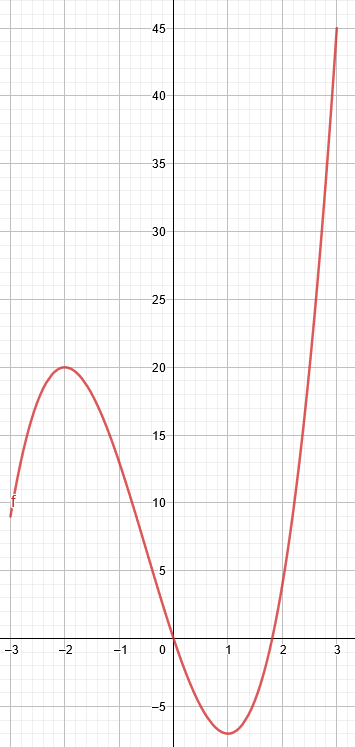
\includegraphics[width=0.9\textwidth]{20221101_CourbeRepTabloVariation.PNG} 
\end{minipage}

Sur la première ligne d'un tableau de variations d'une fonction figurent les antécédents remarquables par la fonction $f$ :\begin{itemize}
    \item Les bornes de l'intervalle où la fonction est définie
    \item Les bornes des intervalles où la fonction est monotone (Ce sont les points où la fonction change de sens de variation)
\end{itemize}

La deuxième partie d'un tableau de variations indique les intervalles croissants par une flèche qui va vers le haut, et les intervalles décroissants par une flèche qui va vers le bas. Puis, on écrit sous les valeurs de la première ligne leurs images par la fonction.


\subsection{Fonctions et équations}

Soit $f$ une fonction définie sur un sous-ensemble des réels, et $a$ un nombre.

\begin{minipage}{0.5\textwidth}  
Résoudre $f(x)=a$ c'est trouver tous les antécédents de $a$ par la fonction $f$.  
\newline ~ \newline
Graphiquement, c'est trouver toutes les abscisses en lesquelles la courbe représentative de la fonction croise la droite horizontale d'ordonnée $a$.
\end{minipage}
\begin{minipage}{0.35\textwidth}
  \begin{tikzpicture}
   \begin{axis}[
	 name = graph1,
     ytick distance = 1,
     xtick distance = 1,
     ymin=-1.1, ymax=6.1,
     xmin=-3.1, xmax=3.1,
     grid=both,
     grid style={line width=.1pt,draw=brown!20},
     major grid style={line width=.2pt,draw=brown!40},
     minor tick num=9,
     tick style={draw=none},
   ]
     \addplot [domain=-10:10, samples=500, color=gray!90]
        {x^2};
     \addplot [domain=-10:10, samples=500, color=blue]
        {3};
     \addplot[only marks, mark=x]coordinates{ (1.73205,3)
		(-1.73205,3)};
      \draw [thick,dashed] (1.73205,0) -- (1.73205,3);
      \draw [thick,dashed] (-1.73205,0) -- (-1.73205,3);
   \end{axis}
   \node[anchor=north][text width=\textwidth][align=center] at (graph1.south) {\scriptsize Résolution graphique de $x^2=3$ :  les deux solutions valent environ $-1.7$ et $1.7$ };
  \end{tikzpicture}
\end{minipage}


\subsubsection{Inéquation}

\begin{de}
    Une \underline{inéquation}, c'est une inégalité entre deux expressions qui s'expriment chacune en fonction d'une même inconnue. Comme dans le cadre d'une équation, \underline{résoudre une inéquation} c'est trouver toutes les valeurs de l'inconnue qui rendent l'inégalité vraie.
\end{de}


\begin{minipage}{0.5\textwidth}  
Résoudre $f(x) \geq a$ c'est trouver tous les antécédents de nombres plus petits que $a$ par la fonction $f$.
\newline ~ \newline
Graphiquement, c'est trouver toutes les abscisses en lesquelles la courbe représentative de la fonction est \textbf{en dessous} de l'ordonnée $a$ (c'est à dire en dessous de la droite d'équation $y=a$.
\newline ~ \newline
A l'inverse, Résoudre $f(x) \geq a$ c'est trouver tous les antécédents de nombres plus grands que $a$ par la fonction $f$.
Graphiquement, c'est trouver toutes les abscisses en lesquelles la courbe représentative de la fonction est \textbf{au dessus} de la droite d'équation $y=a$.


\end{minipage}
\begin{minipage}{0.35\textwidth}
  \begin{tikzpicture}
   \begin{axis}[
	 name = graph1,
     ytick distance = 1,
     xtick distance = 1,
     ymin=-1.1, ymax=2.1,
     xmin=-3.1, xmax=3.1,
     grid=both,
     grid style={line width=.1pt,draw=brown!20},
     major grid style={line width=.2pt,draw=brown!40},
     minor tick num=9,
     tick style={draw=none},
   ]
     \addplot [domain=-10:10, samples=500, color=gray!90]
        {x^2};
     \addplot [domain=-10:10, samples=500, color=blue]
        {1};
     \addplot[only marks, mark=x]coordinates{ (1,1)
		(-1,1)};
      \draw [thick,dashed] (1,0) -- (1,1);
      \draw [thick,dashed] (-1,0) -- (-1,1);
      \draw[red, line width = 3pt] (-1,0) --(1,0); 
        \node[red, line width = 3pt] at (-1,0) {$\Big[$};
        \node[red, line width = 3pt] at (1,0) {$\Big]$};
   \end{axis}
   \node[anchor=north][text width=\textwidth][align=center] at (graph1.south) {\scriptsize Résolution graphique de $x^2 \leq 1$ :  Les solutions valides sont les $x$ de $[-1;1]$ };
\end{tikzpicture}  \begin{tikzpicture}
   \begin{axis}[
	 name = graph1,
     ytick distance = 1,
     xtick distance = 1,
     ymin=-1.1, ymax=2.1,
     xmin=-3.1, xmax=3.1,
     grid=both,
     grid style={line width=.1pt,draw=brown!20},
     major grid style={line width=.2pt,draw=brown!40},
     minor tick num=9,
     tick style={draw=none},
   ]
     \addplot [domain=-10:10, samples=500, color=gray!90]
        {x^2};
     \addplot [domain=-10:10, samples=500, color=blue]
        {1};
     \addplot[only marks, mark=x]coordinates{ (1,1)
		(-1,1)};
      \draw [thick,dashed] (1,0) -- (1,1);
      \draw [thick,dashed] (-1,0) -- (-1,1);
      \draw[red, line width = 3pt] (-3.1,0) --(-1,0);
      \draw[red, line width = 3pt] (1,0) --(3.1,0); 
        \node[red, line width = 3pt] at (-1,0) {$\Big]$};
        \node[red, line width = 3pt] at (1,0) {$\Big[$};
   \end{axis}
   \node[anchor=north][text width=\textwidth][align=center] at (graph1.south) {\scriptsize Les solutions valides de $x^2 \geq 1$ sont les $x$ de $]-\infty;1] \cup [1;+\infty[$ };
  \end{tikzpicture}
\end{minipage}

\subsubsection{Equation $f(x)=g(x)$, Inéquation $f(x) \geq g(x)$}

soient $f$ et $g$ deux fonctions définies sur le même ensemble $E$.

Résoudre $f(x)=g(x)$, c'est trouver tous les nombres qui ont la même image par la fonction $f$ et la fonction $g$. Ca n'est pas très différent que de résoudre $h(x)=0$ quand $h=f-g$ (h est la différence des deux fonctions).

Cependant, il y a une application graphique intéressante qui est souvent demandée en STMG : 

\begin{prop}
    Graphiquement, résoudre $f(x)=g(x)$ si l'on dispose des courbes représentatives de $f$ et de $g$, c'est trouver les abscisses de tous les points où la courbe de $f$ croise la courbe de $g$.

    Graphiquement, résoudre $f(x) \geq g(x)$ si l'on dispose des courbes représentatives de $f$ et de $g$, c'est trouver les abscisses de tous les points où la courbe de $f$ est située au dessus de la courbe de $g$.

\end{prop}

\begin{minipage}{0.5\textwidth}

    Exemple : on voit sur le graphique qui représente sur le même repère nos fonctions exemples $g$ et $h$ que $g(x)=h(x)$ a deux solutions, l'une vaut environ $-0.4$, et l'autre environ $2.4$. Si l'on résoud l'équation algébriquement, on peut trouver que les solutions sont $1-\sqrt{2} \approx -0.414$ et $1+\sqrt{2} \approx 2.414$. Notre approximation graphique est donc utile, d'autant que sur une calculatrice, on peut "zoomer" pour avoir une vision plus précise.
    
    On peut voir que la solution de l'inéquation $g(x) \geq h(x)$ peut être approchée par l'intervalle $[-0.4,2.4]$.  Dans les faits, on vous fera le plus souvent résoudre des équations graphiquement quand les solutions seront directement sur des carreaux de la grille.

    \end{minipage}
    \begin{minipage}{0.45\textwidth}
    
        \centering
        \includegraphics[width=0.9\textwidth]{Geogebra_g(x)=h(x).png} 
    \end{minipage}


\subsection{Sens de variation d'une fonction}

\begin{de}
    Une fonction $f$ est dite \underline{croissante} sur un intervalle $I$ si pour deux nombres $a$ et $b$ de cet intervalle :
    \vspace{0.3cm}
    \begin{center}
    si $a \leq b$,  alors $f(a) \leq f(b)$
    \end{center}
\end{de}

Remarques :
\begin{itemize}
    \item On dit souvent qu'une fonction croissante sur un intervalle conserve l'ordre : Comparer (au sens de "se demander quel nombre est le plus grand") les images de deux éléments donnera le même résultat que comparer ces deux éléments.
    \item Graphiquement, la courbe représentative sur un intervalle "montera" : en parcourant la courbe de gauche à droite, l'image en ordonnée devient de plus en plus haute.
    \item Si l'on peut remplacer les inégalités larges de la définition par des inégalités strictes, on dit que la fonction est \underline{strictement croissante}.
\end{itemize}

Une fonction décroissante, c'est le contraire :

\begin{de}
    Une fonction est dite \underline{décroissante} sur un intervalle $I$ si pour deux nombres $a$ et $b$ de cet intervalle :
    \vspace{0.3cm}
    \begin{center}
    si $a \leq b$,  alors $f(a) \geq f(b)$
    \end{center}
\end{de}

\begin{itemize}
    \item On dit souvent qu'une fonction décroissante sur un intervalle inverse l'ordre : Comparer les images de deux éléments donnera le résultat inverse que comparer ces deux éléments.
    \item Graphiquement, la courbe représentative sur un intervalle "descend" : en parcourant la courbe de gauche à droite, l'image en ordonnée devient de plus en plus basse.
    \item Sur un intervalle donné, une fonction qui est soit décroissante, soit croissante est dite \underline{monotone}. Attention, la fonction doit garder le même sens de variation tout au long de l'intervalle.
    \item Si l'on peut remplacer les inégalités larges de la définition par des inégalités strictes, on dit que la fonction est \underline{strictement décroissante}.
\end{itemize}

\begin{prop}
    Les fonctions affines sont toutes monotones : elles sont croissantes si le coefficient devant le $x$ est positif, et décroissantes sinon.
\end{prop}

La fonction $g(x)=2x+1$ définie plus haut est donc croissante, ce qui se voit bien sur sa représentation graphique.

Contrairement aux fonctions affines que vous aviez vu jusqu'à présent, qui gardaient toujours le même sens de variation, une fonction peut être croissante sur certains intervalles et décroissante sur d'autres. 

Par exemple, la fonction carré est croissante sur $\R^+=[0;+\infty[$ c'est à dire sur les réels positifs et décroissante sur $]-\infty;0]$.  En revanche, on ne peut pas dire qu'elle est monotone sur $\R$, car elle ne reste pas monotone sur l'intervalle. La démonstration est laissée en exercice au lecteur.

\subsection{Fonction affine}

\begin{prop}
    Les fonctions affines (de forme $f(x)=ax+b$ avec $a,b \in \R$) sont les fonctions dont la courbe représentative est une droite. De plus, elles ont un taux de variation constant égal à $a$, entre deux points distincts quelconques.
\end{prop}

Chaque droite qui n'est pas verticale est une représentations de fonctions affines. On peut donc associer à chaque fonction affine $f(x)=ax+b$ 
la droite d'équation $y=ax+b$ qui est sa courbe représentative.

Les coefficients $a$ et $b$ peuvent être lus géométriquement à partir de la droite représentative :
\begin{itemize}
    \item Le coefficient $a$ est la distance verticale (en ordonnée) qui sépare deux points distants de 1 horizontalement (en abscisse). On l'appelle \underline{coefficient directeur} (ou pente) de la droite $y=ax+b$
    \item Le coefficient $b$ est la valeur de la fonction en $0$, c'est donc le point où la droite représentative croise l'axe des abscisses. On l'appelle \underline{ordonnée à l'origine} de la droite
\end{itemize}


Par exemple pour notre fonction $g(x)=2x+1$

\begin{minipage}{0.5\textwidth}
    \begin{tikzpicture} {scale = 3 }
     \begin{axis}[
       name = graph1,
       ytick distance = 1,
       xtick distance = 1,
       ymin=-1.1, ymax=5.1,
       xmin=-1.1, xmax=3.1,
       grid=both,
       grid style={line width=.1pt,draw=brown!20},
       major grid style={line width=.2pt,draw=brown!40},
       tick style={draw=none},
     ]
       \addplot [domain=-10:10, samples=500, color=gray!90]
          {2*x+1};
      \addplot[domain=0:2,samples=3,only marks, mark=x, blue] {2*x+1}; 
      \draw [<->, red] (1,3) -- node[below, red]{$+1$} (2,3);
      \draw [<->, red] (2,3) -- node[right, red]{$+2$} (2,5);
    \end{axis}
     \node[anchor=north] at (graph1.south) {\scriptsize Courbe représentative de $g(x)= 2x+1$  };
    \end{tikzpicture}
\end{minipage}
\begin{minipage}{0.47\textwidth}
    On peut voir que le coefficient $a=2$ est l'augmentation de la droite entre deux points dont l'écart horizontal est de $1$.

    La droite croise la droite des ordonnées au point d'ordonnée $1$, on a donc $b=1$.

\end{minipage}


\subsection{Nombre dérivé, fonction dérivée}

\subsubsection{Taux de variation}

Le taux de variation d'une fonction est défini comme la vitesse à laquelle la fonction croît où décroît entre deux points. 

\begin{de}
    Soit une fonction $f$ définie sur un intervalle contenant deux points $a$ et $b$ distincts. Le taux de variation de la fonction $f$ entre $a$ et $b$ est défini comme le quotient :

    \[ \frac{f(b)-f(a)}{b-a}\]
\end{de}

Note :  C'est le rapport   $\frac{\text{De combien bouge l'image quand la variable passe de a à b?}}{\text{De combien bouge la variable pour passer de a à b?}}$

\begin{prop}
    Les fonctions affines de forme $f(x)=ax+b$ ont un taux de variation constant égal à $a$, entre deux points distincts quelconques.
\end{prop}

En effet, si f est une fonction affine $f : x \mapsto ax+b$, pour tout $x,y \in \R$ tels que $x \neq y$, on a   
\[\frac{f(x)-f(y)}{x-y} = \frac{ax+b-(ay+b)}{x-y} =  \frac{ax+b-ay-b}{x-y} = \frac{a(x-y)}{x-y} = a\]

On en déduit la propriété suivante : il existe toujours une droite qui relie deux points distincts de la courbe représentative d'une fonction,
et on a appris au paragraphe précédent à lire un coefficient directeur de droite. 

\begin{prop}
    Le taux de variation de $f$ entre $a$ et $b$ est le coefficient directeur de la droite qui relie les points d'abscisse $a$ et $b$ de la courbe représentative de $f$.
\end{prop}


\begin{minipage}{0.45\textwidth}
On peut ainsi lire graphiquement le taux de variation d'une fonction entre deux points, en traçant la droite qui relie ces deux points sur la courbe représentative, puis en regardant l'accroissement vertical de la droite entre deux points séparés d'une distance horizontale de 1. 
\vspace{1cm}

Ici, on a tracé en rouge la droite qui relie les points d'abscisse $-1$ et $3$ sur la courbe représentative de la fonction $h(x)=x^2$. La droite rouge représente une fonction dont l'image augmente de $2$ quand on augmente la variable de $1$. 
Elle a donc une pente (ou coefficient directeur) de $2$.  On retrouve bien ce taux d'accroissement en utilisant la formule :  $\frac{h(3)-h(-1)}{3-(-1)}=\frac{9-1}{3+1}=\frac{8}{4}=2$ 
\end{minipage}
\begin{minipage}{0.52\textwidth}
    \begin{tikzpicture}[scale=1.7]
       \begin{axis}[
         name = graph1,
         ytick distance = 1,
         xtick distance = 1,
         ymin=-3.1, ymax=10.1,
         xmin=-6.1, xmax=4.1,
         grid=both,
         major grid style={line width=.2pt,draw=black!40},
         tick style={draw=none}
       ]
         \addplot [domain=-10:10, samples=500, color=blue, line width=1pt]
            {x^2};
         \addplot [domain=-10:10, samples=500, color=red, line width=1pt]
            {(x+1)*2.0 + 1};
         \addplot[only marks, mark size=3pt, mark=x]coordinates{ (-1,1)
            (3,9)};
        \draw [<->, purple] (0,3) -- node[below, purple,scale=.5]{$+1$} (1,3);
        \draw [<->, purple] (1,3) -- node[right, purple,scale=0.5]{$+2$} (1,5);
       \end{axis}
    \end{tikzpicture} 
    \end{minipage}


\subsubsection{Nombre dérivé}

Le nombre dérivé d'une fonction en un point (qu'on appelle aussi dérivée de la fonction en un point) représente le coefficient directeur de la tangente à la courbe représentative de la fonction en ce point. 
On la calcule comme une limite de taux de variation :

\begin{de}
    Soit $f$ une fonction définie sur un intervalle contenant un nombre $a$. Le \underline{nombre dérivé} $f'(a)$ d'une fonction $f$ en $a$ est la limite quand un nombre réel $h$ tend vers 0 de l'expression 

    \[f'(a)=\frac{f(a+h)-f(a)}{h}\]

\end{de}

C'est bien la limite du taux de variation de $f$ entre $a$ et un point très proche de $a$ quand la distance se rapproche de $0$

\begin{prop}
    Si la courbe représentative d'une fonction admet une tangente en un point $a$, le coefficient directeur de cette tangente est donné par le nombre dérivé de la fonction $f$ en $a$.
\end{prop}

\subsubsection{Fonction dérivée}

Au lieu de calculer la tangente en un seul point, on se demande maintenant quel est ce nombre dérivé en chaque point point où $f$ est définie (ou en tout cas sur des intervalles, donc en beaucoup de points)

\begin{de}
    Soit $f$ une fonction définie sur un intervalle $I$ et admettant des nombres dérivés en chaque point de cet intervalle. On appelle fonction dérivée, qu'on note $f'$, la fonction qui à un point associe le nombre dérivé de la fonction en ce point
\end{de}


La tangente d'une courbe représentative nous donne une information capitale sur la fonction : est-elle croissante ou décroissante autour de ce point. On déduit donc de la propriété ci-dessus le théorème fondamental de la dérivée :

\begin{th}
    Soit $f$ une fonction qui admet une fonction dérivée sur un intervalle $I$ :
    \begin{itemize}
        \item $f$ est croissante sur $I$ si et seulement si $f'(x) \geq 0$ pour tout $x$ de $I$ ($f'$ est positive sur $I$)
        \item $f$ est décroissante sur $I$ si et seulement si $f'(x) \leq 0$ pour tout $x$ de $I$ ($f'$ est négative sur $I$)
    \end{itemize}
\end{th}

Remarque : si la dérivée est strictement positive sur $I$, on peut même en déduire que $f$ est strictement croissante sur $I$. Ce n'est pas un "si et seulement si".

\subsubsection{Dérivées de fonctions connues}

En première STMG, vous avez appris, en plus de la définition d'un nombre dérivé, à calculer les dérivées de : 

\begin{tabular}{|l|c|c|c|}
    \hline
    Nom de la fonction & Expression& Degré & Fonction dérivée \\
    \hline
    Fonction constante& $f(x) = x^0 = 1$ & $0$ & $f'(x)=0$ \\
    \hline
    Fonction identité& $f(x) = x^1 = x$ & $1$ & $f'(x)=1$ \\
    \hline
    Fonction constante& $f(x) = x^2$ & $2$ & $f'(x)=2x$ \\
    \hline
    Fonction constante& $f(x) = x^3$ & $3$ & $f'(x)=3x^2$ \\
    \hline
\end{tabular}

Vous avez également appris à calculer la dérivée des combinaisons linéaires de ces fonctions, c'est à dire que vous savez que :\begin{enumerate}
    \item Produit par une constante : Pour un réel $k$, et une fonction $f$ dérivable de dérivée $f'$ : la dérivée de la fonction $kf$ qui à $x$ associe $k\times f(x)$ est égale à $kf'$
    \item La dérivée de la somme de deux fonctions est la somme des dérivées : $(f+g)' = f'+g'$
\end{enumerate}


\section{Fonction exponentielle}

\subsection{Rappels sur les puissances}

\subsubsection{puissances entières positives}

On sait depuis la troisième calculer les puissances entières positives d'un nombre $a$.

\begin{de}
    Soit $a$ un nombre, et $n$ un entier positif. La quantité $a^n$ (prononcée "a puissance n") est le nombre :

    \[
        \underbrace{a \times a \times \dots \times a \times a}_{\text{Le nombre $a$ apparaît $n$ fois}}  
    \]
\end{de}

Exemples :  \begin{itemize}
    \item $7^1 = 7$.
    \item $7^2 = 7 \times 7$. On appelle $a^2$ a au carré (c'est l'aire d'un carré de côté $a$ si $a>0$).
    \item $7^3 = 7 \times 7 \times 7$. On appelle $a^3$ a au cube (c'est le volume d'un cube de côté $a$ si $a>0$).
    \item $10^5 = 10 \times 10 \times 10 \times 10 \times 10 = 100\,000$. En général, $10^n$ vaut le chiffre  $1$ suivi de $n$ zéros.  
\end{itemize}


Les pusisances ont des propriétés agréables avec la multiplication : Par exemple, si l'on essaye de calculer $2^4 \times 2^3$ :

\begin{tabular}{ccc}
    $2^4$ & $\times$ & $2^3$ \\
    \multicolumn{3}{c}{On utilise la formule de la puissance}\\
    $\underbrace{2 \times 2 \times 2 \times 2}_{\text{Le nombre $2$ apparaît $4$ fois}}$& $\times $ & $\underbrace{2 \times 2 \times 2}_{\text{Le nombre $2$ apparaît $3$ fois}}$\\ 
    \multicolumn{3}{c}{Au final, on a un produit où le terme 2 apparaît $4+3$=7 fois}\\
    \multicolumn{3}{c}{$\underbrace{2 \times 2 \times 2 \times 2 \times 2 \times 2 \times 2 }_{\text{Le nombre 2 apparaît 7 fois}}$}\\
    \multicolumn{3}{c}{Ceci vaut (toujours par la définition) : }\\
    \multicolumn{3}{c}{$2^7$}\\
      
\end{tabular}

Cette propriété reste vraie pour n'importe quel nombre dont on fait la puissance, et n'importe quelles puissances:

\begin{prop}
    pour $a \in \R$ et $n,m \in \N$, on a :   $a^n \times a^m = a^{n+m}$
\end{prop}


Une autre propriété utile est quand on met un produit à une certaine puissance :

\begin{tabular}{rcl}
$(2 \times 3)^4$&$ =$&$ (2 \times 3)  \times (2 \times 3)  \times (2 \times 3) \times (2 \times 3)$ \\
& $=$ & $2 \times 3  \times 2 \times 3  \times 2 \times 3 \times 2 \times 3$ \\
& $=$ & $2 \times 2  \times 2 \times 2  \times 3 \times 3 \times 3 \times 3$\\
& $=$ & $(2 \times 2  \times 2 \times 2)  \times (3 \times 3 \times 3 \times 3)$\\
& $=$ & $2^4  \times 3^4$\\
\end{tabular}

Cette propriété est également vraie pour toutes les valeurs des nombres :

\begin{prop}
    pour $a \in \R$, $b \in \R$ et $n \in \N$, on a :   $(a \times b)^n = a^{n} \times b^n$
\end{prop}

\subsubsection{puissances nulles et négatives} 

La première propriété vue au-dessus nous assure que $2^{n+1} = 2 \times 2^n$. 
On voit donc que pour passer d'une puissance de $2$ à la puissance suivante, on multiplie par 2 (c'est littéralement une suite géométrique). 
On peut donc passer d'une puissance à la puissance précédente en divisant par $2$, c'est à dire en multipliant par $\frac{1}{2}$ : $2^2 = 2^3 \times \frac{1}{2}$

On peut donc compléter le tableau dans les deux sens (vers la droite, mais aussi vers la gauche), en partant de $2^1=2$ 

{
\centering
    \begin{tabular}{|c|c|c|c|c|c|}
        \hline
        $2^{-2}$ & $2^{-1}$ & $2^0$ & $2^1$  & $2^2$ & \ldots \\
        \hline
         $\frac{1}{2\times 2} = \frac{1}{4} = \frac{1}{2^2}\insertph{n1}$ & $\insertph{n2}\frac{1}{2}\insertph{n3}$ & $\insertph{n4}\frac{2}{2}=1\insertph{n5}$ & $\insertph{n6}2\insertph{n7}$ &  \ $\insertph{n8}2 \times 2 = 4$  & \ldots \\ 
        \hline
    \end{tabular}\par
}

\tikz[remember picture,overlay]\draw[<-,red] ([yshift=-2mm] n1.south) to  [out=-45,in=-150] node[below]{$\times \frac{1}{2}$} ([yshift=-2mm] n2.south) ; 
\tikz[remember picture,overlay]\draw[<-,red] ([yshift=-2mm]n3.south) to[out=-45,in=-150] node[below]{$\times \frac{1}{2}$}  ([yshift=-2mm]n4.south); 
\tikz[remember picture,overlay]\draw[<-,red] ([yshift=-2mm]n5.south) to[out=-45,in=-150] node[below]{$\times \frac{1}{2}$} ([yshift=-2mm]n6.south); 
\tikz[remember picture,overlay]\draw[->,blue] ([yshift=-2mm]n7.south) to[out=-45,in=-150] node[below]{$\times 2$} ([yshift=-2mm]n8.south); 
\vspace{20 mm}

On remarque qu'on peut étendre la définition d'une puissance aux nombres nuls et négatifs :  $2^0$ est égal à $1$. 

De plus, pour tout entier $n$, $2^{-n}=\frac{1}{2^n}$

Cette propriété reste vraie pour tout nombre non nul dont on prend une puissance : 

\begin{prop}
    Pour tout nombre $a$ non nul, et tout entier $n$ positif :

    \[ a^0 = 1\]

    \[ a^{-n} = \frac{1}{a^n} \]
\end{prop}

Note : Les propriétés $a^{n+m} = a^n a^m$  et $(ab)^n = a^n b^n$, vues plus haut, restent vraies pour n nul ou négatif, quand ces expressions sont bien définies.

On remarque notamment qu'en utilisant la première propriété, on a pour tout nombre $a$ non nul : 

$a^{n} \times a^{-n} = a^{n+(-n)} = a^0 = 1$.   On a donc $a^n \times a^{-n} = 1$, ce qui est la même chose que de dire que $a^{-n} = \frac{1}{a^n}$. 

\subsubsection{Puissances non-entières}

On a maintenant étendu à toutes les valeurs entières de $n$ la définition de $a^n$,  que $n$ soit positif ou négatif. 
Maintenant, on veut étendre cette définition même aux valeurs non entières. Pour ne pas l'étendre n'importe comment, on veut que cette extension préserve 
la précieuse égalité :  $a^(x+y) = a^x \times a^y$

Commençons doucement : Que pourrait valoir le nombre $x = 2^{\frac{1}{2}}$ ?   Si on utilise la première propriété, et qu'on met $x$ au carré, on obtient :

\[ x^2 = 2^{\frac{1}{2}} \times 2^{\frac{1}{2}} = 2^{\frac{1}{2} + \frac{1}{2}} = 2^1 = 2\]

$2^{\frac{1}{2}}$ mis au carré vaut donc 2.  Il est donc légitime d'attribuer à $2^{\frac{1}{2}}$ la valeur de $\sqrt{2}$

En utilisant cette méthode, on peut attribuer une valeur à $a^x$ pour toute valeur positive de $a$, et pour toute valeur rationnelle de $x$. On peut ensuite étendre à toute valeur réelle de $x$ pour obtenir les fonctions exponentielles

\subsection{Fonction exponentielle}

\begin{de}
    Soit $a$ un nombre réel strictement positif. On appelle \underline{fonction exponentielle de base $a$} la fonction définie sur $\R$ :

    \[ \begin{array}{ccccc}
        \text{exp}_a & : & \R & \to & \R \\
         & & x & \mapsto & a^x \\
        \end{array}\]
\end{de}


\begin{prop}
    Les propriétés des puissances entières restent vraies pour les puissances non entières pour $a$ et $b$ réels positifs,  et $x,y$ réels quelconque : 
    \begin{multicols}{2}
        \begin{enumerate}
            \item $a^{x+y} = a^x \times a^y$
            \item $a^{-x} = \frac{1}{a^x}$
            \item $a^{xy} = (a^{x})^y$
            \item $(ab)^{x} = a^{x}b^x$
        \end{enumerate}
    \end{multicols}
\end{prop}


\begin{minipage}{0.4\textwidth}
    \begin{tikzpicture}
     \begin{axis}[
       name = graph1,
       ytick distance = 1,
       xtick distance = 1,
       ymin=-1.1, ymax=16.1,
       xmin=-6.1, xmax=5.1,
       grid=both,
       grid style={line width=.1pt,draw=brown!20},
       major grid style={line width=.2pt,draw=brown!40},
       tick style={draw=none},
     ]
  
       \addplot [domain=-10:10, samples=500, color=red!90]
          {2^x};
      \addplot[domain=1:10,samples=10,only marks, mark=x, blue] {2^x}; 
     \end{axis}
     \node[anchor=north] at (graph1.south) {\scriptsize Courbe représentative de $exp_2(x)= 2^x$  };
    \end{tikzpicture}
\end{minipage}
\begin{minipage}{0.58\textwidth}
    Une fonction exponentielle de base $a$ est en fait le prolongement d'une suite géométrique de raison $a$ à toutes les valeurs non réelles : 
    \begin{itemize}
        \item les croix bleues du graphique à gauche sont les termes de la suite $u_n = 2^n$ pour $n \leq 1$
        \item La courbe rouge est la courbe représentative de la fonction exponentielle de base 2 : qui à $x$ associe $2^x$
    \end{itemize}
\end{minipage}

\subsubsection{Sens de variation et courbe représentative}

Il n'est pas surprenant que le sens de variation d'une fonction exponentielle soit la même que celle 
d'une suite géométrique. 

\begin{prop}[Sens de variation de la fonction exponentielle $x \mapsto a^x$]
Quand le nombre $a$ est strictement supérieur à $1$, la fonction exponentielle de base $a$  
est strictement croissante. 

Quand le nombre $a$ est égal à 1, la fonction est constante.

Quand le nombre $a$ est strictement compris entre 0 et 1, la fonction est décroissante.
\end{prop}

\begin{minipage}{0.32\textwidth}
    \begin{tikzpicture}
     \begin{axis}[
       name = graph1,
       ytick distance = 1,
       xtick distance = 1,
       ymin=-1.1, ymax=10.1,
       xmin=-5.1, xmax=5.1,
       grid=both,
       grid style={line width=.1pt,draw=brown!20},
       major grid style={line width=.2pt,draw=brown!40},
       tick style={draw=none},
     ]
  
       \addplot [domain=-10:10, samples=500, color=red!90]
          {1.5^x};
     \end{axis}
     \node[anchor=north] at (graph1.south) {\scriptsize Courbe représentative de $x \mapsto 1{,}5^x$  };
    \end{tikzpicture}
\end{minipage}
\begin{minipage}{0.32\textwidth}
    \begin{tikzpicture}
     \begin{axis}[
       name = graph1,
       ytick distance = 1,
       xtick distance = 1,
       ymin=-1.1, ymax=10.1,
       xmin=-5.1, xmax=5.1,
       grid=both,
       grid style={line width=.1pt,draw=brown!20},
       major grid style={line width=.2pt,draw=brown!40},
       tick style={draw=none},
     ]
  
       \addplot [domain=-10:10, samples=500, color=blue!90]
          {1^x};
     \end{axis}
     \node[anchor=north] at (graph1.south) {\scriptsize Courbe représentative de $exp_1(x)= 1^x = 1$  };
    \end{tikzpicture}
\end{minipage}
\begin{minipage}{0.32\textwidth}
    \begin{tikzpicture}
     \begin{axis}[
       name = graph1,
       ytick distance = 1,
       xtick distance = 1,
       ymin=-1.1, ymax=10.1,
       xmin=-5.1, xmax=5.1,
       grid=both,
       grid style={line width=.1pt,draw=brown!20},
       major grid style={line width=.2pt,draw=brown!40},
       tick style={draw=none},
     ]
     =
       \addplot [domain=-10:10, samples=500, color=green!90]
          {.66667^x};
     \end{axis}
     \node[anchor=north] at (graph1.south) {\scriptsize Courbe représentative de $exp_{\frac{2}{3}}(x)= \frac{2}{3}^x$  };
    \end{tikzpicture}
\end{minipage}


\subsubsection{Produit d'une exponentielle par une constante}

Quand on multiplie une fonction par une constante $k$:
\begin{itemize}
    \item Si $k$ est positif, la fonction conserve son sens de variation
    \item Si $k$ est négatif, la fonction change de sens de variation (Une fonction croissante devient décroissante et vice-versa)    
\end{itemize}

\begin{minipage}{0.5\textwidth}
    Dans le cas de la fonction exponentielle :
    \begin{itemize}
        \item Si $k$ est positif, la fonction conserve son sens de variation
        \item Si $k$ est négatif, la fonction change de sens de variation (Une fonction croissante devient décroissante et vice-versa)    
    \end{itemize}

    Ci-contre, $1{,}1 > 1$ donc $exp_{1{,}1}$ est croissante.  $2$ étant positif et $-2$ négatif, la fonction $f_1(x)= 2 \times {1,1}^x$ est strictement croissante
    et la fonction $f_2(x)= -2 \times {1,1}^x$ est décroissante.
\end{minipage}
\begin{minipage}{0.4\textwidth}
    \begin{tikzpicture}
     \begin{axis}[
       name = graph1,
       ytick distance = 1,
       xtick distance = 1,
       ymin=-5.1, ymax=5.1,
       xmin=-10.1, xmax=10.1,
       grid=both,
       grid style={line width=.1pt,draw=brown!20},
       major grid style={line width=.2pt,draw=brown!40},
       tick style={draw=none},
     ]
  
       \addplot [domain=-10:10, samples=500, color=red!90]
          {2 * 1.1^x};
        \addplot [domain=-10:10, samples=500, color=blue!90]
             {-2 * 1.1^x};
     \end{axis}
     \node[anchor=north] at (graph1.south) {\scriptsize Courbe représentative de $f_1(x)= 2 \times {1,1}^x$ et $f_2(x)= -2 \times {1,1}^x$  };
    \end{tikzpicture}
\end{minipage}



\section{Fonction logarithme}

\subsection{Fonction réciproque}

Parfois, juste en connaissant l'image d'un nombre par une certaine fonction, on peut deviner ce nombre. 




\end{document}